\documentclass[11pt]{article}

%  USE PACKAGES  ---------------------- 
\usepackage{float}
\usepackage{enumitem}
\setlist[itemize]{noitemsep, topsep=0pt}
\usepackage[margin=0.7in,vmargin=1in]{geometry}
\usepackage{amsmath,amsthm,amsfonts}
\usepackage{amssymb}
\usepackage{fancyhdr}
\usepackage{fancyvrb}
\usepackage{enumerate}
\usepackage[T1]{fontenc}
\usepackage{mathtools}
\usepackage{graphicx}
\usepackage{tcolorbox}
\usepackage{hyperref,color}
\usepackage{enumitem,amssymb}
\newlist{todolist}{itemize}{4}
\setlist[todolist]{label=$\square$}
\usepackage{pifont}
\fvset{fontsize=\small,fontfamily=times}
\newcommand{\cmark}{\ding{51}}%
\newcommand{\xmark}{\ding{55}}%
\newcommand{\done}{\rlap{$\square$}{\raisebox{2pt}{\large\hspace{1pt}\cmark}}%
\hspace{-2.5pt}}
\newcommand{\HREF}[2]{\href{#1}{#2}}
\usepackage{textcomp}
\usepackage{listings}
\lstset{
basicstyle=\small\ttfamily,
% columns=flexible,
upquote=true,
breaklines=true,
showstringspaces=false
}
%  -------------------------------------------- 

%  HEADER AND FOOTER (DO NOT EDIT) ----------------------
\pagestyle{fancy}
\fancyhead{}
\newcommand{\newquestion}[1]{
\clearpage % page break and flush floats
\renewcommand{\problemnumber}{#1} % set problem number for header
\phantom{}  % Put something on the page so it shows
}
\fancyfoot[L]{IE 332}
\fancyfoot[C]{Project Submission}
\fancyfoot[R]{Page \thepage}
\renewcommand{\footrulewidth}{0.4pt}

%  --------------------------------------------


%  COVER SHEET (FILL IN THE TABLE AS INSTRUCTED IN THE ASSIGNMENT) ----------------------
\newcommand{\addcoversheet}{
\clearpage
\thispagestyle{empty}
\vspace*{0.5in}

\begin{center}
\Huge{{\bf IE332 Project \#2}} % <-- replace with correct assignment #

Due: April 28th, 11:59pm EST % <-- replace with correct due date and time
\end{center}

\vspace{0.3in}

\noindent We have {\bf read and understood the assignment instructions}. We certify that the submitted work does not violate any academic misconduct rules, and that it is solely our own work. By listing our names below we acknowledge that any misconduct will result in appropriate consequences. 

\vspace{0.2in}

\noindent {\em ``As a Boilermaker pursuing academic excellence, I pledge to be honest and true in all that I do.
Accountable together -- we are Purdue.''}

\vspace{0.3in}

\begin{table}[h!]
  \begin{center}
    \label{tab:table1}
    \begin{tabular}{c|ccccc|c|c}
      Student & Algorithm & Complexity & Implementation & Testing & Report & Overall & DIFF\\
      \hline
      Matt Fortier & 40 & 20 & 10 & 15 & 15 & 100 & 0\\
      Geoffrey Ladue & 15 & 20 & 10 & 15 & 40 & 100 & 0\\
      Josiah Mann & 15 & 20 & 10 & 40 & 15 & 100 & 0\\
      Anthony Matejko & 15 & 20 & 35 & 15 & 15 & 100 & 0\\
      Shamam Tabindah & 15 & 20 & 35 & 15 & 15 & 100 & 0\\
      \hline
      St Dev & 11 & 0 & 14 & 11 & 11 & 0 & 0
    \end{tabular}
  \end{center}
\end{table}

\vspace{0.2in}

\noindent Date: \today.
}
%  -----------------------------------------

%  TODO LIST (COMPLETE THE FULL CHECKLIST - USE AS EXAMPLE THE FIRST CHECKED BOXES!) ----------------------


%% LaTeX
% Für alle, die die Schönheit von Wissenschaft anderen zeigen wollen
% For anyone who wants to show the beauty of science to others

%  -----------------------------------------


\begin{document}


\addcoversheet
\pagebreak
\tableofcontents
\pagebreak

\section{Main Text}

\subsection{Algorithms}

\noindent 

\subsection{Extended Research \& Attempted Methods}

\noindent Although we implemented the algorithms outlined in Section 1.1, the team devoted significant time to researching common methods of adversarial attacks and even generated corresponding alternatives in RStudio. These attempted methods, while unsuccessful upon implementation, are a worthwhile case study in the team's product development.

\subsubsection{Random Pixel Flip}

\noindent Random pixel flipping generates perturbed images that can be used to confuse a machine learning model. The idea behind this technique is to flip the value of one or more pixels in an image to create a new image that is similar to the original image but that the machine learning model will classify differently.\\

\noindent From the team's research, the main advantage of random pixel flipping is that it is a simple and efficient way to generate a large number of adversarial examples quickly. By randomly flipping a small number of pixels in an image, the algorithm can generate many different perturbed images that are all slightly different but still belong to the same class. This makes it difficult for the machine learning model to distinguish between the original image and the perturbed images.\\

\begin{center}
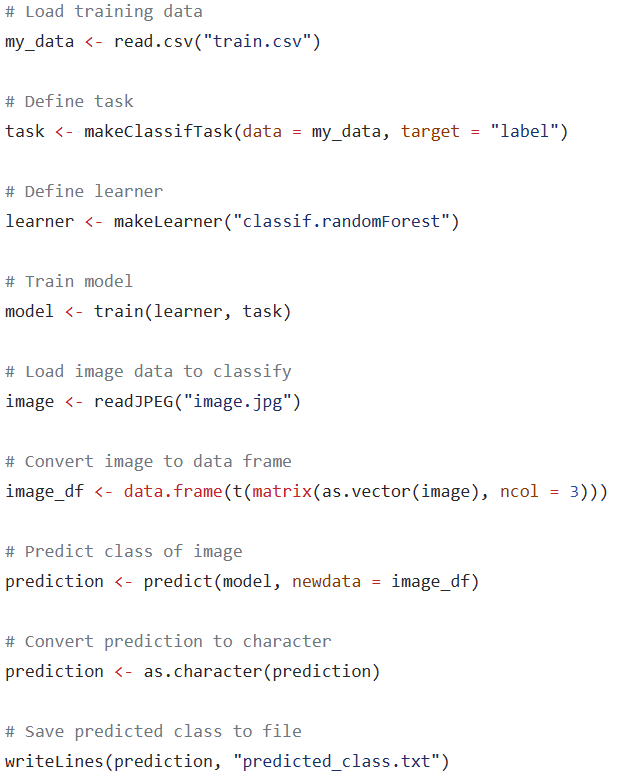
\includegraphics[scale=.75]{PixelFlip.png}\\
\textbf{Figure : Pixel Flip Algorithm}
\end{center}

\noindent The algorithm described in the Figure \_ code works by first calculating the number of pixels to flip based on the image dimensions and the budget specified by the user. It then generates a set of perturbed images by randomly flipping the specified number of pixels in the original image using the generate\_perturbed\_images() function. It then applies the classify\_image() function to each perturbed image using the map() function from the purrr library to classify the image.\\

\noindent Finally, the algorithm counts the number of occurrences of each class among the perturbed images using the table() function and returns the most common class using the which.max() function. This allows the algorithm to determine which class the machine learning model is most likely to predict for the perturbed images, even though they are all slightly different from the original image.\\

\noindent Overall, random pixel flipping can be a useful tool for adversarial attacks because it allows an attacker to generate a large number of perturbed images quickly and efficiently, making it difficult for a machine learning model to accurately classify the images. This can be particularly useful in situations where an attacker wants to trick a machine learning model into making a specific prediction.

\subsubsection{Decision Trees}

\begin{center}
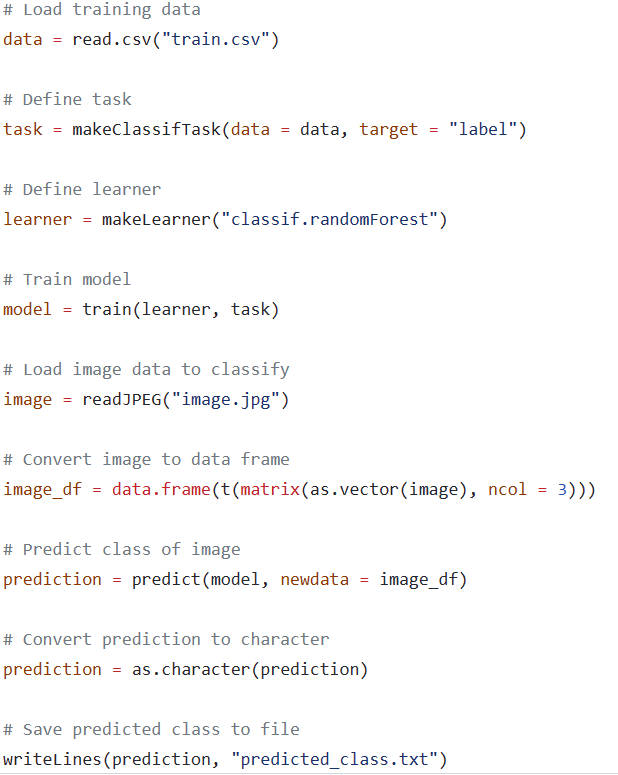
\includegraphics[scale=.75]{DecisionTree.png}\\
\textbf{Figure : Decision Tree Algorithm}
\end{center}

\noindent The team also researched Random Forest algorithms in depth to determine if it would be suitable to explore decision tree-based solutions. The code outlined in Figure \_ is a powerful tool for image classification tasks. The use of parallel processing helps to speed up the computation time, allowing for faster model training and classification. By defining a classification task using the makeClassifTask() function and creating a learner object using makeLearner(), the algorithm is able to train sample data and learn patterns within it that can be used for classification. Once the model is trained, it can accurately predict the class of new images. This makes it a useful tool for adversarial attacks, as it can be used to identify vulnerabilities in image classification systems and create adversarial images that can bypass security measures. The ability to quickly and accurately classify images using Random Forest makes it an important tool for image classification in a variety of settings.

\subsubsection{Fast Gradient Sign Method with Vector Machine Classifier}

\noindent The team found the Fast Gradient Sign Method (FGSM) method to be the most popular and effective attack method for generating adversarial examples. The FGSM attack works by calculating the gradient of the model's loss function with respect to the input image, and then perturbing the image in the direction of the gradient to maximize the loss. This perturbation is controlled by a hyper parameter, epsilon, which determines the magnitude of the perturbation added to the image.\\

\begin{center}
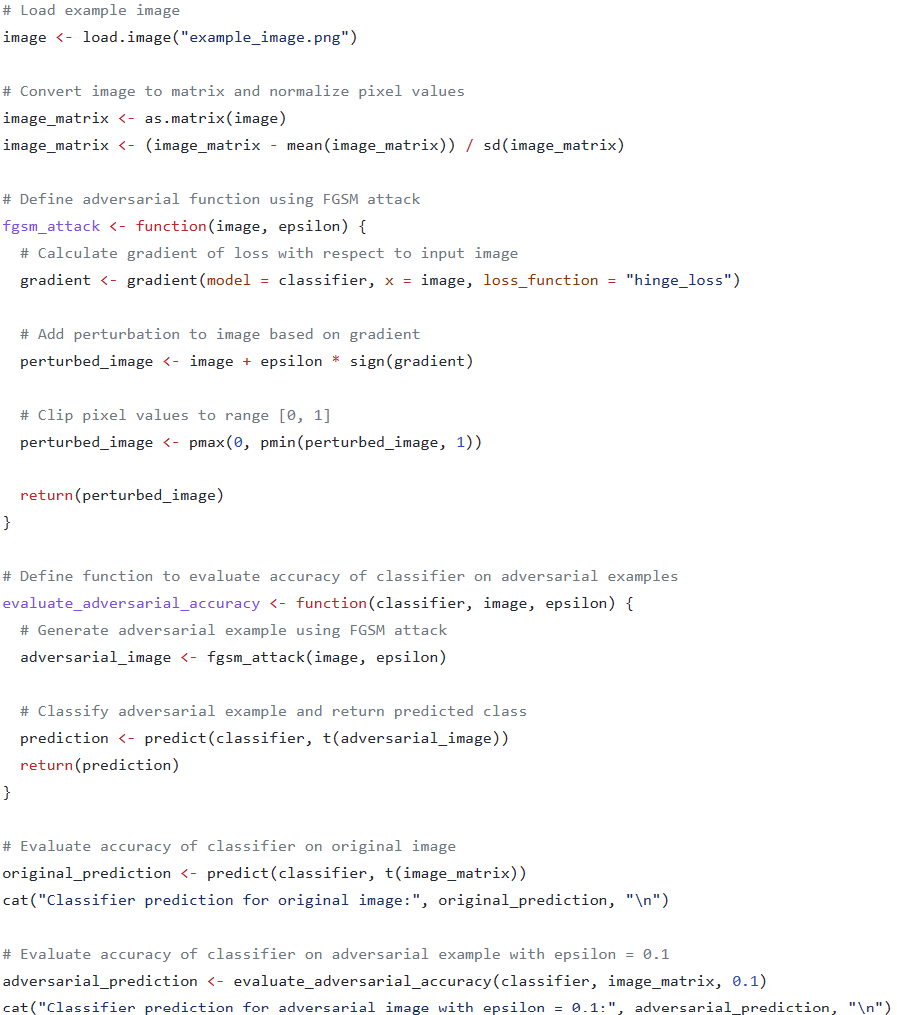
\includegraphics[scale=.75]{FGSM1.png}\\
\textbf{Figure : FGSM w/ Vector Machine Classifier Algorithm}
\end{center}

\noindent The code in Figure \_ generates adversarial examples using the FGSM attack, and evaluates the accuracy of a pre-trained support vector machine (SVM) classifier on both the original and adversarial images. The code loads the pre-trained SVM classifier and an example image, and normalizes the pixel values of the image matrix. It then defines a function called fgsm\_attack() to generate adversarial examples using the FGSM attack. The perturbed image is obtained by adding a scaled version of the gradient to the original image. The pixel values of the perturbed image are clipped to the range [0, 1].\\

\noindent The evaluate\_adversarial\_accuracy() function takes in the SVM classifier, an image, and an epsilon value, and returns the predicted class label for the adversarial image generated by the fgsm\_attack() function. This function calls fgsm\_attack() to generate the adversarial image, and then predicts the class label using the predict() function.\\

\noindent FGSM is a useful tool for evaluating the robustness of a pre-trained SVM classifier to adversarial attacks generated using the FGSM method. By generating adversarial examples and evaluating the accuracy of the classifier on both the original and adversarial images, we could have utilized FGSM to assess the vulnerability of the classifier to such attacks and develop more robust models.

\subsubsection{Stack Generalization}

\begin{center}
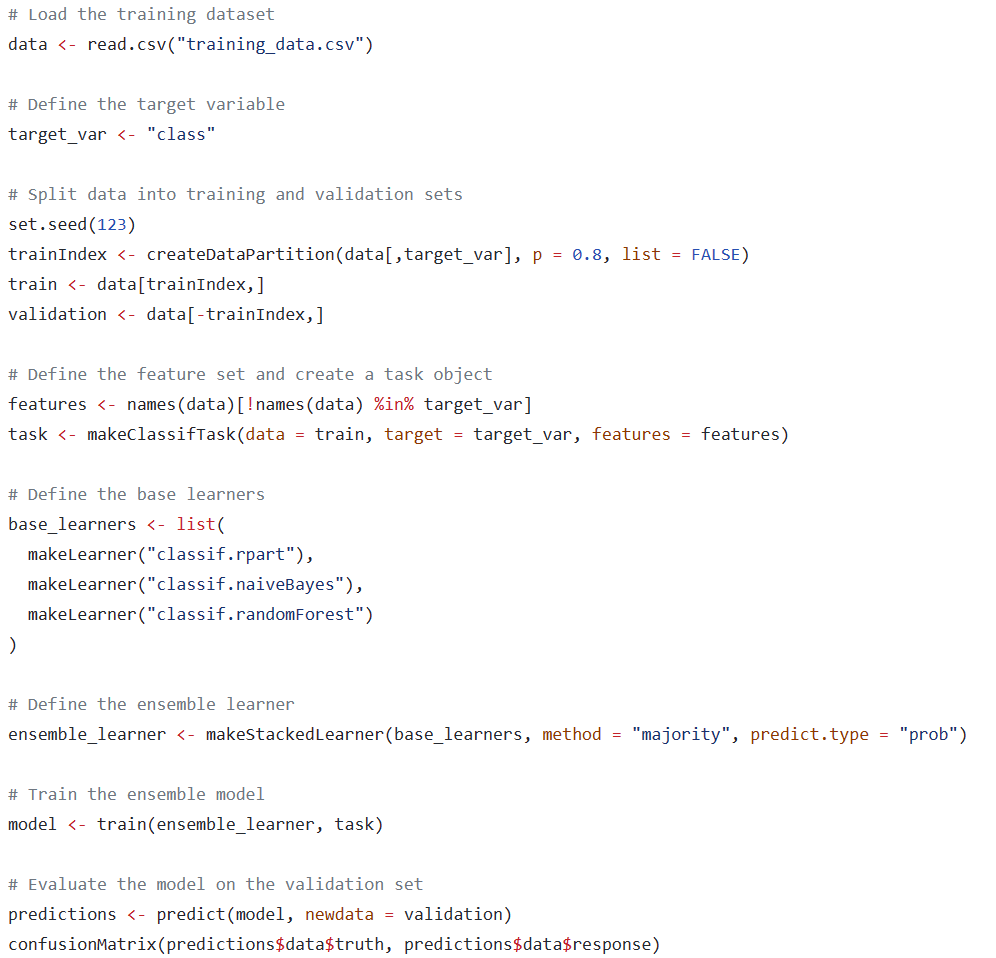
\includegraphics[scale=.75]{StackGen.png}\\
\textbf{Figure : Stack Generalization Algorithm}
\end{center}

\noindent The ensemble learning method used Figure \_'s code can be a useful tool for the purpose of adversarial attacks as it combines multiple models to improve the accuracy of the classifier, which can make it more robust against adversarial attacks. The base learners used in this code, including a decision tree, a naive Bayes classifier, and a random forest, were combined through the team's research since they are known to be susceptible to adversarial attacks. By combining them in an ensemble, the resulting model may be less vulnerable to such attacks. Additionally, by using the validation set to evaluate the performance of the model, the code can identify potential weaknesses or vulnerabilities in the model, which can be used to improve its robustness against adversarial attacks. While this method was unsuccessful, this was the team's attempt to integrate multiple algorithm methods.

\subsubsection{Second Fast Gradient Sign Method}

\noindent The algorithm described in the Figure \_'s generates an adversarial example using the Fast Gradient Sign Method (FGSM) attack mentioned in Section 1.2.3, but without a vector machine classifier.\\

\noindent The code uses the Keras library to load a pre-trained image classification model from an HDF5 file and defines an epsilon value. It then defines a function called generate\_adversarial, which takes the pre-trained model, input image, target label, and epsilon value as input. This function calculates the loss and gradients of the model with respect to the input image, calculates the sign of the gradients, and perturbs the input image in the direction of the sign of the gradients. Finally, it clips the perturbed input data to ensure it remains within the valid range of [0, 1].\\

\noindent The generated adversarial example can be useful for testing the robustness of a pre-trained model to adversarial attacks. Adversarial examples are known to fool deep neural networks, and evaluating the performance of a model on both the original and adversarial examples can provide insights into the model's vulnerabilities to adversarial attacks.

\begin{center}
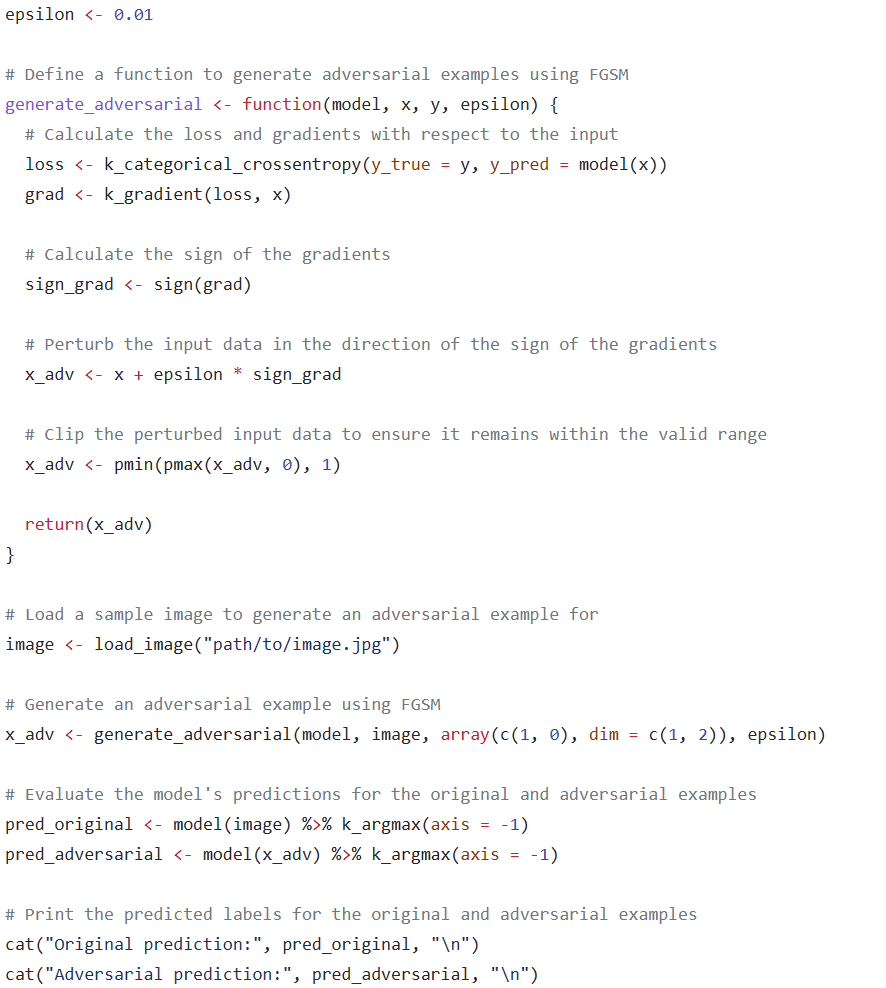
\includegraphics[scale=.75]{FGSM2.png}\\
\textbf{Figure : FGSM Algorithm}
\end{center}

\pagebreak

\section{Appendices}

\subsection{Testing / Correctness / Verification}

% 0.01 is defualt value for pixel budget

% Matt wants to make list of pixels to change and run accordingly

% try different pixel budgets for each subalg and running individually to see what percent could be fooled to verify correctness of subalg

Extensive verification and testing was performed on each of the sub-algorithms used to modify the images, themselves, in order to verify that the main model, and thus main goals, of this project were sufficiently met. Our groups approach to verifying the correctness of each sub-algorithm consisted of running each program with varying pixel budgets to ensure that we received the correct output. Furthermore, each program was run individually within the main model to ensure that the percent the algorithm was fooled was as we had previously predicted.

% try and actually perform testing to get images if R works

\noindent Testing was also performed on our main algorithm as well to verify that it too produced our intended results. In order to do so, we simply had to run our main algorithm with standard parameter inputs for both our main algorithm as well as the parameter values that were passed to the various sub-algorithms that were discussed previously. Fortunately, the group was able to achieve success very quickly once each of the sub-algorithms had been verified for correctness.

\subsection{Run-time Complexity and Wall-time}

When it comes to run-time complexity our algorithms all use the quantile (type 1) algorithm. This function is very commonly used in real-world databases. The quantile algorithm has, at worst, a run-time complexity of O($n^2$). Since our algorithms involve loops that iterate over an array, we can see that the outer loop iterates n times and the inner loop also iterates n times giving us our total iterations being $n^2$. Our algorithms have the run-time complexity of O($n^2$) which grow quadratically with the size of input. With this run-time complexity, the larger the input, the slower the algorithm will work.

\subsection{Performance}

Shamam

\subsection{Justification}

\subsubsection{Alternative Weighting Method}

\begin{center}
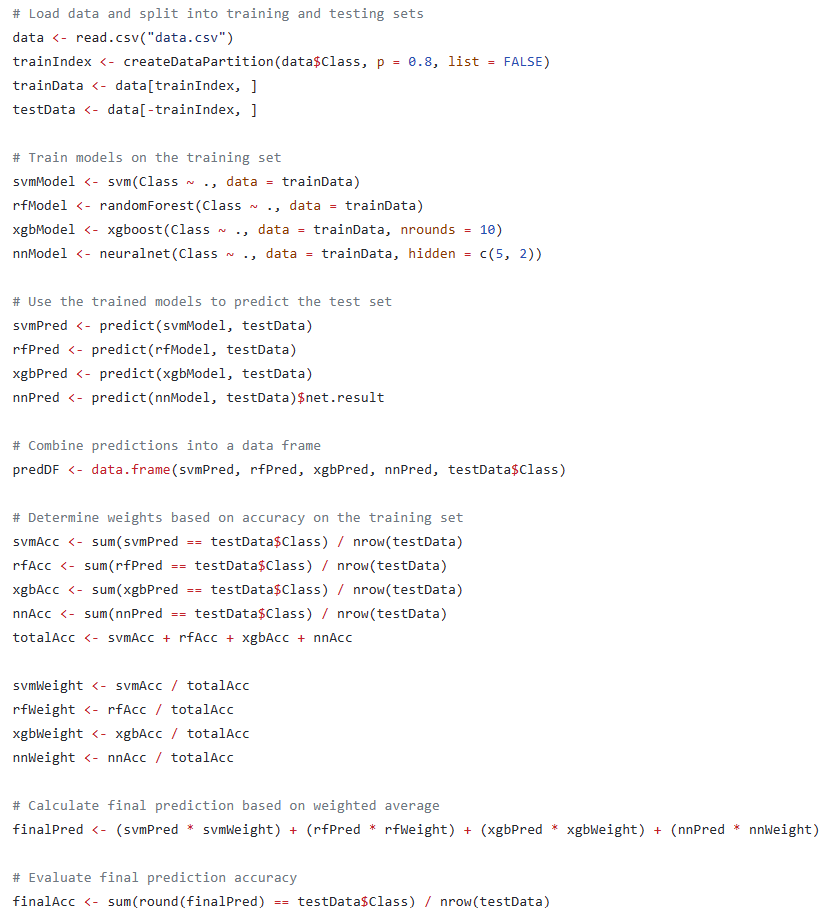
\includegraphics[scale=.75]{WeightAlgo.png}\\
\textbf{Figure : Alternative Weighting Algorithm}
\end{center}

\noindent As outlined in Section 1.2, the team researched potential methods for adversarial attack implementation. As such, a corresponding weighting algorithm was generated as a test case for how the team would be alternatively solved the problem at hand. The code shown in Figure \_ is useful for weighting adversarial attack algorithms because it combines multiple models with different strengths to improve the accuracy of predictions. The use of a weighted average to combine the predictions of the models allows for a more flexible and adaptable system than the final product discussed in Section 2.4. The weights are determined based on the accuracy of the individual models on the testing set, meaning that the weights can change depending on the dataset being used. This allows the system to adjust to different types of attacks and datasets, potentially making it more resilient against a wider range of adversarial attacks.

\end{document}

